%%%%%%%%%%%%%%%%%%%%%%%%%%%%%%%%%%%%%%%%%
% Medium Length Professional CV
% LaTeX Template
% Version 3.0 (December 17, 2022)
%
% This template originates from:
% https://www.LaTeXTemplates.com
%
% Author:
% Vel (vel@latextemplates.com)
%
% Original author:
% Trey Hunner (http://www.treyhunner.com/)
%
% License:
% CC BY-NC-SA 4.0 (https://creativecommons.org/licenses/by-nc-sa/4.0/)
%
%%%%%%%%%%%%%%%%%%%%%%%%%%%%%%%%%%%%%%%%%
% https://www.latextemplates.com/template/medium-length-professional-cv 

%----------------------------------------------------------------------------------------
%	PACKAGES AND OTHER DOCUMENT CONFIGURATIONS
%----------------------------------------------------------------------------------------

\documentclass[
	a4paper, % Uncomment for A4 paper size (default is US letter)
	11pt, % Default font size, can use 10pt, 11pt or 12pt
]{resume} % Use the resume class

\usepackage{ebgaramond} % Use the EB Garamond font
\usepackage{fontawesome5}

\usepackage{hyperref}
\hypersetup{
    colorlinks=true,
    linkcolor=blue,
    filecolor=magenta,      
    urlcolor=cyan,
    %pdftitle={Overleaf Example},
    %pdfpagemode=FullScreen,
    }

\urlstyle{same}

\usepackage{graphicx}
\graphicspath{ {./} }
%------------------------------------------------

\name{Sebin Shaji Philip} % Your name to appear at the top
%\MakeUppercase{\textbf{Sebin Shaji Philip}}

% You can use the \address command up to 3 times for 3 different addresses or pieces of contact information
% Any new lines (\\) you use in the \address commands will be converted to symbols, so each address will appear as a single line.

%\address{sebin@kth.se • +91 9496990284 • linkedin.com/in/sebinsphilip/ • India}
\address{\faIcon{envelope} sebin@kth.se\hspace{2ex}\faIcon{whatsapp} +91 9496990284\hspace{2ex}\faIcon{linkedin} linkedin.com/in/sebinsphilip/\hspace{2ex}\faIcon{globe} India}
%\address{123 Broadway \\ City, State 12345} % Main address

%\address{123 Pleasant Lane \\ City, State 12345} % A secondary address (optional)

%\address{(011)~$\cdot$~899~$\cdot$~9881 \\ john@LaTeXTemplates.com} % Contact information

%----------------------------------------------------------------------------------------

\begin{document}

%----------------------------------------------------------------------------------------
%	EDUCATION SECTION
%----------------------------------------------------------------------------------------

\begin{rSection}{Education}
    \begin{rSubsection}{Università di Trento}{September 2020 - July 2022}{Master of Science in Embedded Systems}{Trento, Italy}

        Courses: Real-time OS and middleware, Low power wireless networking for IoT, Robot planning and its applications. Research project on implementing Nonvolatile processor architecture (NVP for energy harvesters) on RISC-V core (ibex). (Minor: Entrepreneurship for Engineers, Business Development Lab)
    
        {\color{orange}\emph{Intermittent Computing Emulation of Ultra-Low-Power Processors: Evaluation of Backup Strategies for RISC-V} - IEEE Transactions on Computer-Aided Design of Integrated Circuits and Systems, April 20, 2022} \href{https://ieeexplore.ieee.org/document/9760506}{[view]}.
    \end{rSubsection}

    \begin{rSubsection6}{KTH Royal Institute of Technology}{September 2019 - July 2022}{Master of Science in Embedded Systems}{Stockholm, Sweden}{Armada Career Host}{EIT Digital Excellent Scholarship (C1)}

        Courses: Embedded Software (Realtime, Parallel computing and Models of Computation using ForSyDe), Computer Systems Architecture, Compilers and Execution Environments, Embedded Systems (HW SW co-design, Real-Time model and Priority driven scheduling, RTOS, Embedded Computing Platform).
    \end{rSubsection6}
    
    \begin{rSubsection5}{TKMCE, University of Kerala}{September 2012 - April 2016}{Bachelor of Technology in Computer Science and Engineering.}{Kerala, India}{First Class with Distinction, GPA: 8.4/10}

        Courses: Digital Systems Design, Operating Systems and Network Programming, Data Structures and Algorithms, Microprocessor and Interfacing, High Performance Microprocessors, Digital Signal Processing, Distributed Systems, Digital Image Processing, Computer Graphics, Unix Systems Programming.\hfill
        \bigskip\break
        {\color{orange}[Thesis] Entity Level Contextual Sentiment Detection of Topic Sensitive Influential Twitterers using SentiCircles. \break
        IC3T Springer Journal: Published in 2016 \href{https://link.springer.com/chapter/10.1007/978-981-10-3223-3\_19}{[view]}\hfill \break
        Best project: Computer Society of India 5th In-App award} \hfill

    
    \end{rSubsection5}
    
	%Minor in Linguistics \smallskip \\
		
\end{rSection}

%----------------------------------------------------------------------------------------
%	WORK EXPERIENCE SECTION
%----------------------------------------------------------------------------------------

\begin{rSection}{Experience}
%------------------------------------------------

    \begin{rSubsection}{Thales}{August 2022 - December 2022}{Software Engineer}{Vienna, Austria}
        Involved in the support of TAS Control Platform (safety-critical fault-tolerant platform) as part 
        of Thales Railway Signalling Solutions team. Contributed fixes towards TAS control platform NTP/Chrony time 
        synchronization implementation and focused on TAS Core OS/Target handling work.
		
    \end{rSubsection}

%------------------------------------------------
	\begin{rSubsection}{KAI (Kompetenzzentrum Automobil- und Industrieelektronik), Infineon}{October 2021 - June 2022}{Master thesis student}{Villach, Austria}

            {\color{orange} Zephyr RTOS: Design of a Deterministic Ethernet Network for Machine-to-Machine (M2M) Communications}\href{https://www.linkedin.com/in/sebinsphilip/overlay/1635506986689/single-media-viewer/?type=DOCUMENT&profileId=ACoAAAm-xe0BCYwezV-q9pIlhl7WYDQHRff8kIE}{[view]}: Thesis involve (i) writing complete XMC4 ethernet driver for Zephyr RTOS, supporting IEEE1588(PTP), VLAN tagging and DMA operations. (ii) Implementing timer, counter, clock and other peripheral driver and devicetrees of XMC for Zephyr (iii) Integrating network stacks like UDP, TCP, MQTT and MQTT-SN of Zephyr with ethernet (iv) integrating gPTP Zephyr stack for network time synchronization (IEEE 802.1AS) (v) Implementing real-time traffic shaping algorithms based on IEEE 802.1Qav (credit-based stream reservation) and investigate feasibility of IEEE802.1Qbv on XMC4.
            \href{https://github.com/sebinsphilip/zephyr\_xmc}{ See code here.}
		
	\end{rSubsection}

%------------------------------------------------

	\begin{rSubsection}{ThinkSeed Systems}{August 2021 - October 2021}{Embedded Software Consultant}{Remote}
            Design and develop android system services and C++ (JNI) layer for Apple wireless carplay stack interacting with Accessory (Automotive/Car dashboard) and iPhone (device). Including designing and implementing services and its state machines to maintain resource manager (BT, Audio, Video), wireless connection etc. (Ref: Apple Accessory Interface Specification: CarPlay, MFi etc.)

		
	\end{rSubsection}

%------------------------------------------------

	\begin{rSubsection}{WindMachines AB}{July 2020 - December 2020}{Embedded Software Engineer(intern)}{ Stockholm, Sweden}
            Developing battery controller (charger/balancer) for Li-Ion and Pb-Acid batteries on a AVR based microcontroller (ATMEGA32L) for novel Savonius Vertical axis wind turbines (50W – 2KW).

	\end{rSubsection}
 
%------------------------------------------------

	\begin{rSubsection}{StepUp Air}{April 2020 - July 2020}{Embedded Software Engineer(intern)}{ Copenhagen, Denmark}
            Part of an early stage 2-member Embedded team responsible for developing code for ‘StepUp Air’, a breath measuring wearable for athletes. Technologies include BLE, ANT+, DFU, BOOTLOADER for Nordic Semiconductors nRF52 SoC.

	\end{rSubsection}
 
%------------------------------------------------

	\begin{rSubsection}{Hewlett-Packard Enterprise}{October 2018 - July 2019}{Firmware Engineer II}{India}
            Part of a dedicated 3-member team responsible for maintaining and do feature addition for firmware of HPE Apollo Gen10 server chassis controller (part of Baseboard Management Controller). Tasks include maintaining communication in RTOS via I2C, SPI etc., modifying cooling (fan/PWM), power regulation (PID controller) and BSP for new firmware requirements.
            %\hspace{1em} % Vertical whitespace after the end of the list
            %\break \break

            [server] Instant Power Reporting - MQTT Daemon: Designed and implemented an MQTT daemon (using PowerPC cross-compiled mosquitto libs) on Linux initrd. This daemon exposed a very simple universal interface to communicate over TCP/IP (ethernet). Periodically reporting power(instant) events from the server tray controller to the central Power management unit(dashboard) was a use-case. It made use of both Apache Avro and JSON format as payloads.
            %\vspace{1em} % Vertical whitespace after the end of the list
            %\break \break
            
            Maintain firmware/state-machine of on-board chassis MegaCell (battery) on Smart-Array-Controller for HPE
Apollo Gen10 servers.


	\end{rSubsection}
 %------------------------------------------------

	\begin{rSubsection}{AllGo Embedded Systems, Visteon Corp.}{July 2016 - Oct 2018}{Embedded Software Engineer}{India}
            Part of multimedia and connectivity team responsible for requirement gathering, developing, documenting and bug fixing of the Embedded Linux based automotive multimedia stack as well as the connectivity stack for Tier1 automotive OEM companies.
            %\hspace{1em} % Vertical whitespace after the end of the list
            %\bigskip\break

            Designed and Implemented WiFiPlugin for Wireless CarPlay and AndroidAuto device detection and connection. The library implementation made use of DNS-SD (Bonjour) protocol for service discovery and Hostapd for Wireless Access point management in Embedded Linux. (TATA Q5 Infotainment project) \hfill
            %\vspace{1em} % Vertical whitespace after the end of the list
            %\bigskip\break
            
            Enabled direct playback from Android phone without using a device-driver: Removed complete device-driver dependency for MTP device read/write from MTP library(libmtp/linux) and redirect them into direct user-space(libusb) operations as part of AOSP project. Also implemented buffering feature for reducing read-latency and thus smooth audio playback music playback from MTP device. (Mitsubishi Infotainment project) \hfill
            %\bigskip\break

            Design and implementation of Automotive MediaPlayer WAMP-C++ Binder layer (autobahn-cpp/bonefish) on top of CommonAPI(C++) layer for streamlining communication over JavaScript and C++. This implementation provides direct RPC calls as JSON message formats from WebInterface(JavaScript) to the underlying stack (CommonAPI/C++).
            %\bigskip\break

            Created and optimised gstreamer pipelines as part of codec/container validation on Renesas/imx platform and implemented audio-book/podcast support for embedded Sqlite3 based mediaplayer in C.

	\end{rSubsection}
%------------------------------------------------

	\begin{rSubsection}{QBurst Technologies}{May 2015 - June 2015}{Intern}{India}
            Designed and developed iOS app to calculate dimensions of an object (length x width) using iPhone camera in Objective-C.
            \href{https://github.com/sebinsphilip/The\_Dimension\_Tool} {See code here.}

	\end{rSubsection}
 
\end{rSection}

%----------------------------------------------------------------------------------------
%	TECHNICAL STRENGTHS SECTION
%----------------------------------------------------------------------------------------

\begin{rSection}{Technical Strengths}

	\begin{tabular}[t]{m{3cm} m{14cm}}
		\textbf{Tools} & gcc, gdb, GNU Make, CMake, lcov, Coverity, cpp-lint, git, svn, RTC, Gerrit, IAR
Workbench, Quartus Prime, ModelSim, Altera NiosII Qsys, MATLAB \\
            \textbf{OS} & Linux/Ubuntu, Zephyr RTOS, Contiki, ThreadX, uCOS-II \\
            \textbf{Programming} & C, C++, Bash shell scripting, Python, VHDL, System Verilog \\
		\textbf{Leadership skills} & mentored and guided junior engineers for knowledge transfer, also collaborated with different R\&D teams to gather all available resources/knowledge for designing embedded applications from scratch.

	\end{tabular}
 
\end{rSection}

%----------------------------------------------------------------------------------------
%	PROJECTS
%----------------------------------------------------------------------------------------

\begin{rSection}{Projects}

	%Section content\ldots
        \item {[UniTrento]} Course project of ‘Low power wireless networking for IoT’, for developing ‘Time Synchronization and Periodic Data Collection’ protocol on Contiki OS. Task involve developing time synchronized period data collection for wireless network nodes (with efficient duty-cycling for achieving low power – MAC layer), generating routing topology, scheduling transmissions and wakeups etc.\href{https://github.com/sebinsphilip/LowPowerWN\_IOT}{ [view]}
        \item {} \href{https://github.com/sebinsphilip/zephyr\_xmc}{Master thesis code repo}, which contains the out-of-tree drivers developed for the thesis. The main ethernet driver code can be found \href{https://github.com/sebinsphilip/zephyr\_xmc/tree/main/drivers/zephyr/ethernet}{here}.
        \item {} A simple POSIX shell implemented using a state machine \href{https://github.com/sebinsphilip/matician\_shell}{[view]}.
        \item {} HackerRank and IEEE Xtreme coding challenges \href{https://github.com/sebinsphilip/coding\_challenge}{[view]}.
        \item {[KTH]} Parallel Multi-core (5-cores) implementation of Edge detection filters (Image processing) on Altera Nios II FPGA using bare metal and uCOS-II RTOS. Throughput requirement of 320 images per second (32x32 pixels). Involved Design space exploration of different actors and mapping different tasks on multiple processors considering real-time (deadline) requirements and utilizing parallel programming constructs. \href{https://github.com/sebinsphilip/Embedded\_software\_lab} {[view]}
        \item {[KTH]} Implemented efficient Vedic multipliers on FPGA for high performance cryptographic applications. \href{https://github.com/sebinsphilip/vedic\_multiplier\_kth\_writing\_course}{[view]}
        \item {[hobby-project]} Implemented gstreamer based music playback application on Linux. The Linux userspace music player opened and played an OGG file in PC to alsasink by creating a filesrc-oggdemux- vorbisdec-alsasink pipeline in Gstreamer.
        \href{https://github.com/sebinsphilip/gstreamer\_applications}{[view]}
        \item {[hobby-project]} Basic USB device driver to read/write to bulk endpoint as part of Device driver study. \href{https://github.com/sebinsphilip/device\_drivers}{[view]}
        \item {[hobby-project]} Multi-client (with username) supported TCP chat server as part of Socket programming study. \href{https://github.com/sebinsphilip/sockets}{[view]}

\end{rSection}

%----------------------------------------------------------------------------------------

%----------------------------------------------------------------------------------------
%	REFERENCES
%----------------------------------------------------------------------------------------

\begin{rSection}{LANGUAGE}
%\centering (Available upon request)
	%Section content\ldots
    \item {ENGLISH (CEFR C1 Level): } [IELTS Jan 2019] Listening(8) Reading(8.5) Writing(7) Speaking(7.5), Overall (8/9)
    \item {GERMAN (CEFR A1 Level) : }  Overall (48/60) 
    \item {MALAYALAM              : } Native or bilingual proficiency
\end{rSection}

%----------------------------------------------------------------------------------------

%----------------------------------------------------------------------------------------
%	SAMPLES OF WORK
%----------------------------------------------------------------------------------------

\begin{rSection}{CONTACT INFORMATION}
    \centering 
        %Section content\ldot
        \begin{tabular}[t]{m{3.5cm} m{14cm}}
        Sebin Shaji Philip,
        Kuruvanthanam (House),
        Paingana,
        Mundakayam P.O.,
        Kottayam, Kerala
        India,
        PIN: 686513 & 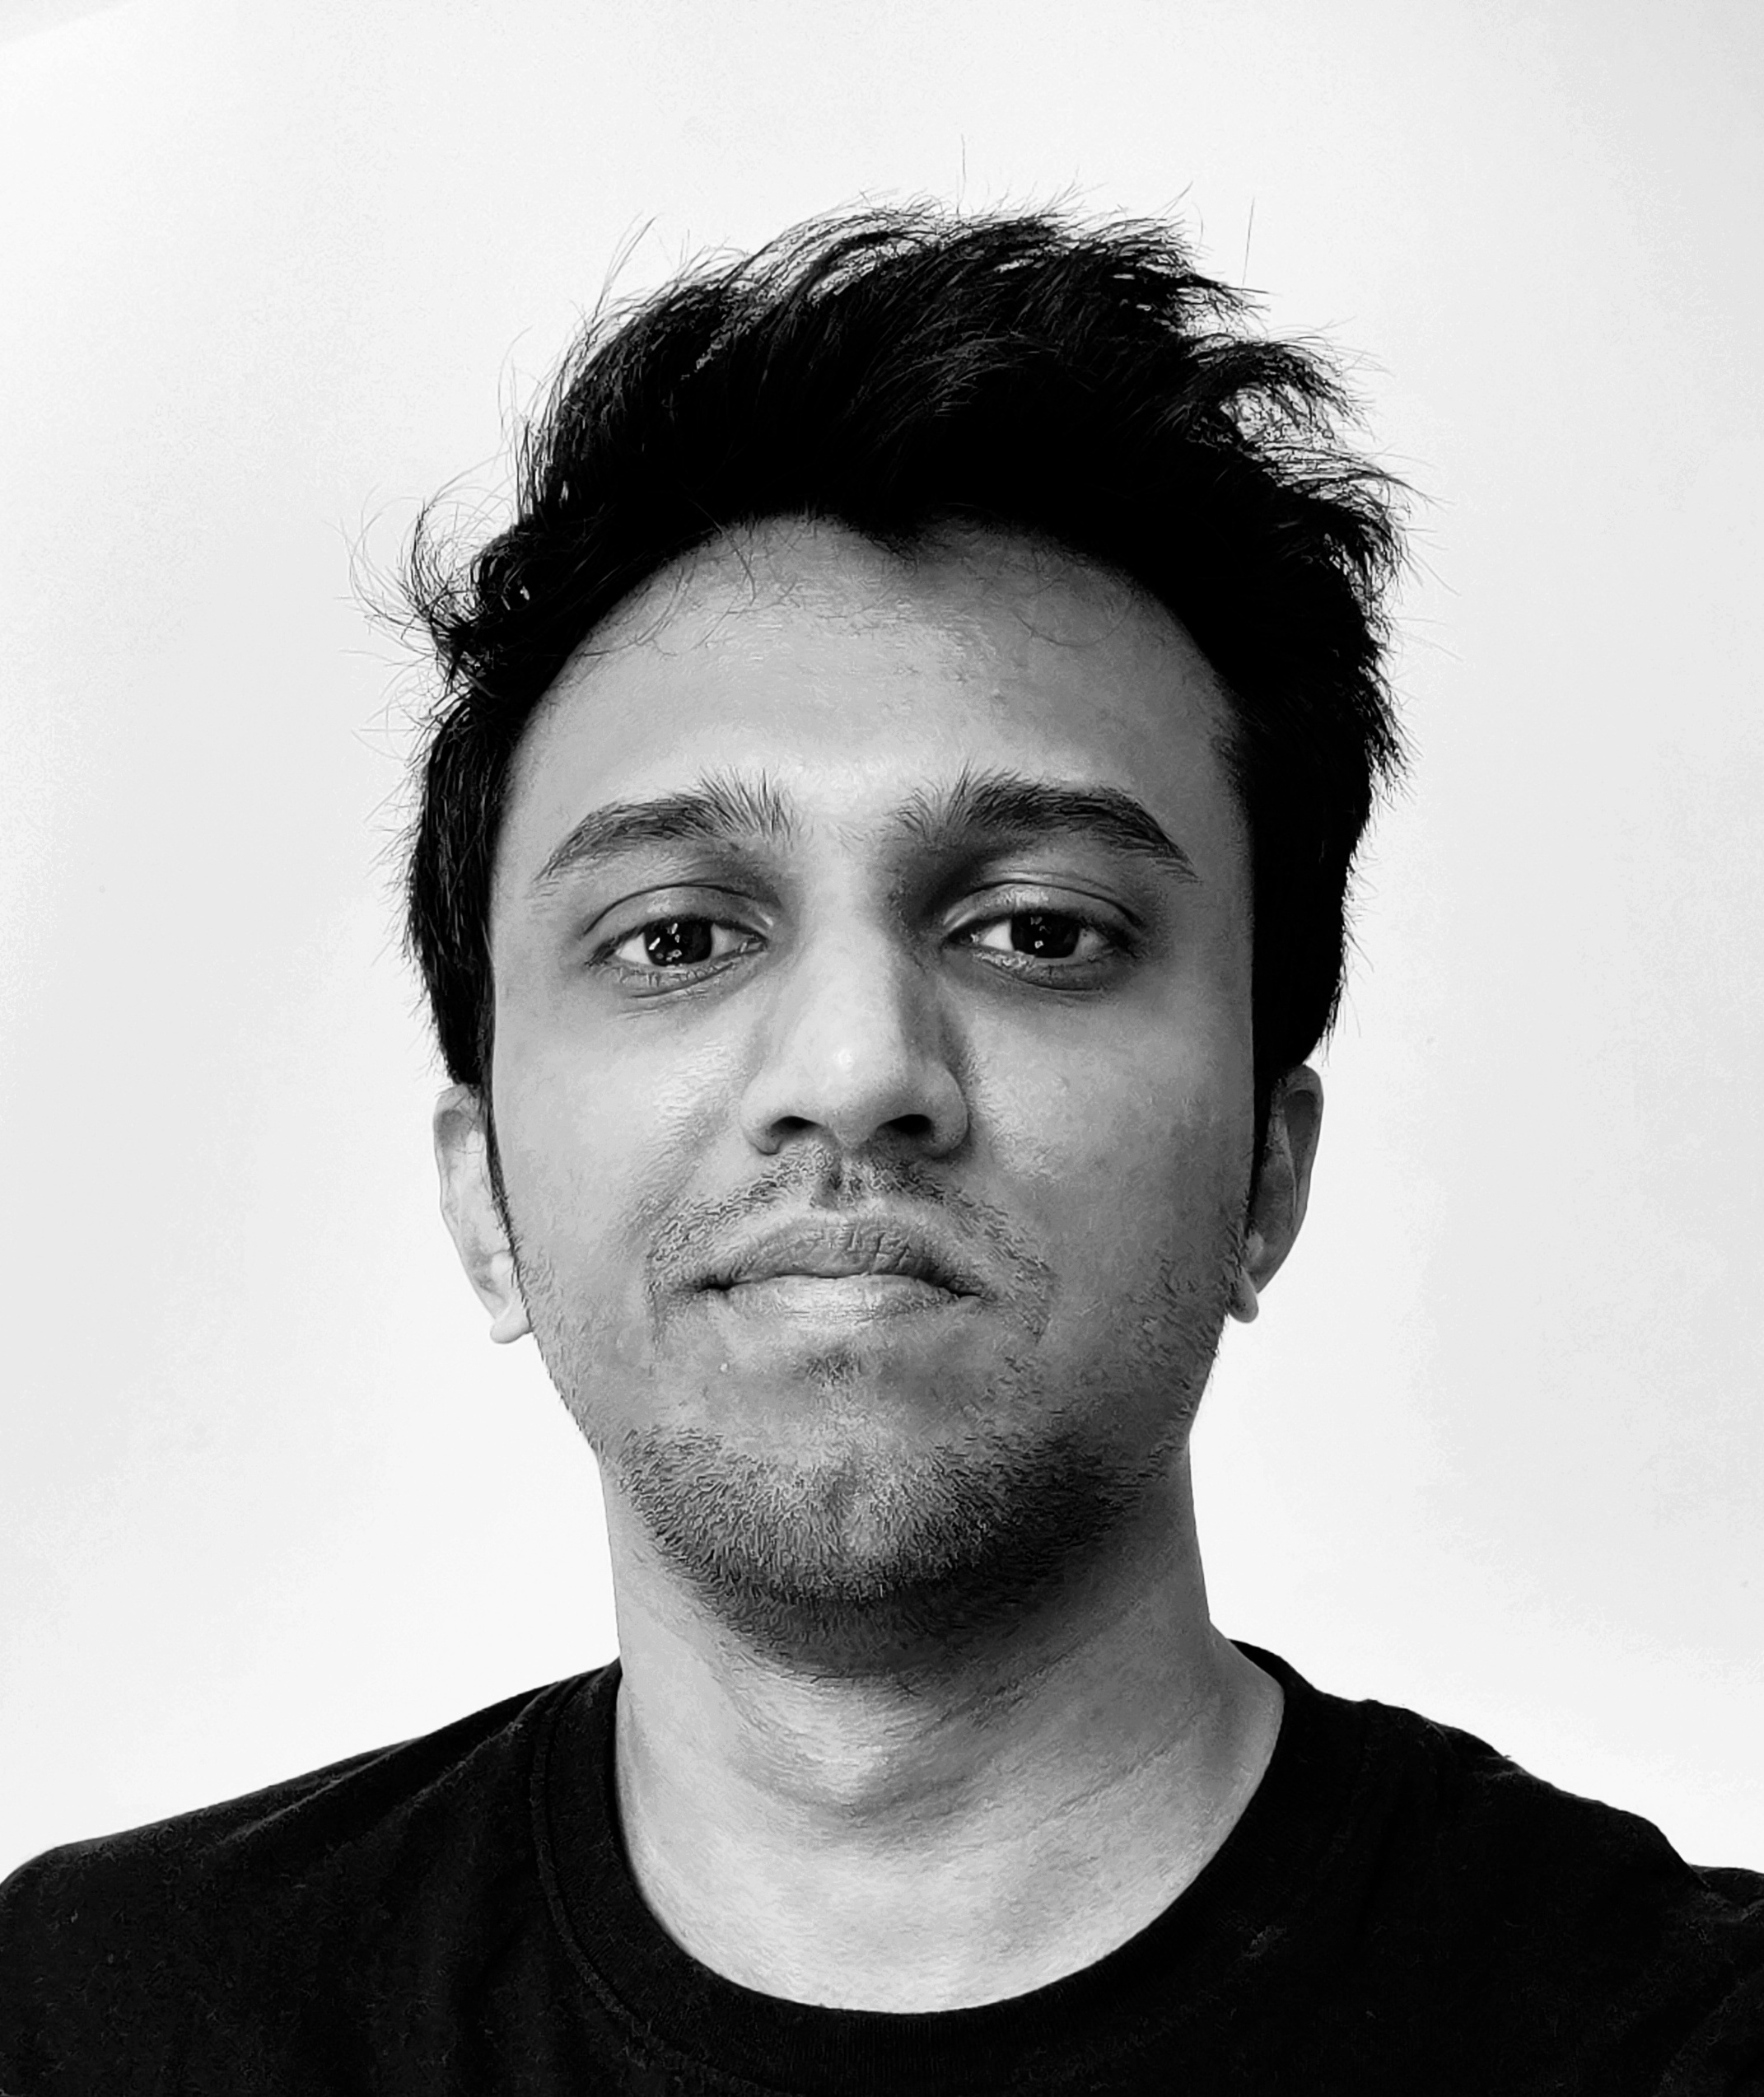
\includegraphics[width=3.5cm, height=4cm]{dp}
        \end{tabular}
        
        
    \end{rSection}
    
    %----------------------------------------------------------------------------------------
    
\end{document}
